\chapter{Minimax Agent}

In the world of artificial intelligence and game strategies, the minimax algorithm is a key method for making decisions when competing against others.
The main idea of minimax is to predict and counter the opponent's moves while trying to maximize its own advantage.
At its core, the minimax algorithm operates on the principle of recursively exploring the game tree, considering all possible moves by both players 
up to a certain depth or until a terminal state is reached. Each node in the tree represents a game state, and the algorithm assigns a value to 
each node based on the potential outcome of the game from that state. The key idea driving minimax is the assumption that the opponent will make 
moves that are optimal for them, aiming to minimize the agent's potential gain.

While minimax is powerful, it is also a heuristic-based approach. It doesn't guarantee finding the optimal solution but rather approximates it by 
searching through the game tree. Despite its effectiveness, minimax does have limitations, primarily related to the vast branching factor of certain game trees, 
which can lead to exponential growth in computation as the depth increases. 

While minimax excels in deterministic games like chess, its application becomes more complex in games with imperfect information, 
where players have limited or incomplete knowledge about the game state or their opponents' actions. In non-deterministic games, traditional minimax 
strategies struggle due to the inability to accurately assess the state space. Unlike deterministic games where the entire game state is known, 
non-deterministic games introduce uncertainty, making it difficult for the agent to construct a comprehensive game tree.

In this chapter, I delve into the implementation of minimax specifically adapted for Sagrada. I discuss how I approached challenges such as 
high branching factors and imperfect information within the context of Sagrada's gameplay mechanics. By detailing my approach to integrating minimax into 
the game's decision-making process while addressing these factors, I aim to provide valuable insights into the development of AI agents for complex board games.

\section{Branching Factor}

As discussed in Section \ref{subsec:smarter_player_branching_factor} , it's evident that smarter players exhibit markedly different branching factors compared to random agents.
In the case of minimax agents, the branching factor tends to be significantly higher because the heuristic function guides the player towards more promising moves. This results
in choosing moves that make space for higher branching factor in the following turns because it rarely chooses moves that produce uncompletable fields and fields that 
are completable with only a small amount of different dice. The following figure visualizes the average branching factor over 1000 games for a minimax and a random agent:

\begin{figure}[H]
    \caption{ Branching factor comparison between the minimax agent and the random agent}
    \centerline{\mbox{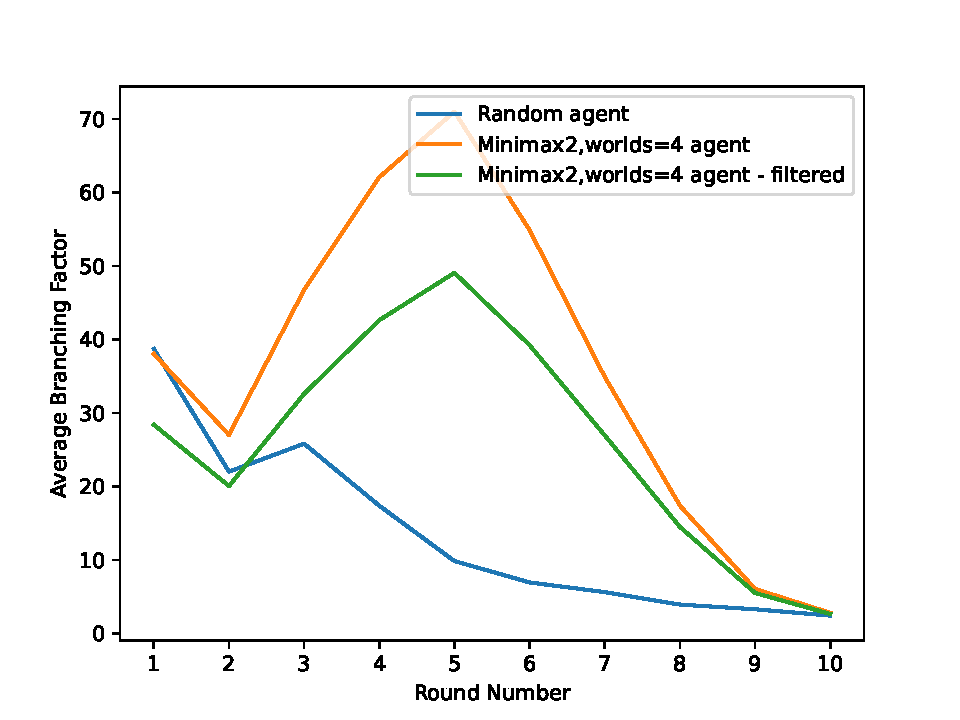
\includegraphics[width=180mm]{img/minimax_agent_branching_factor.pdf}}}
    \label{fig:example}
\end{figure}


\section{The Algorithm}

At its core, the minimax algorithm operates on the premise of minimizing the possible loss for a worst-case scenario while simultaneously maximizing potential gains. 
It's particularly effective in two-player, zero-sum games, where each player aims to outmaneuver the other. 

The game's possible future states are represented as a game tree, with each node denoting a possible move by a player. In Sagrada, a game with a high branching factor, 
this tree can rapidly expand, making exhaustive search impractical.  Each terminal node or leaf of the game tree is assigned a heuristic value, 
reflecting the desirability of that game state for the player. Starting from the terminal nodes, these values are propagated upwards through the tree. 
Generally, at each level, the algorithm alternates between maximizing and minimizing the values, simulating the moves of both players. 
For a comprehensive overview of the minimax algorithm, see \cite{enwiki:1217764079}.


This works for games where the players make moves one after the other. Note that in Sagrada choosing the minimizing and the maximizing player for the next layer is not 
that straightforward because the players do not strictly alternate moves. Also, the implementation of some Tool Cards consists of multiple sub-moves as described in Section 
\ref{subsec:Move_Implementation}  making the choice of the next level's playing strategy even harder. 

To explore the state nodes of the game tree, I am using the pre-processed possible moves using the heuristic filter already described in Section
\ref{sec:Heuristic_filter} . This is one of the ways I am dealing with the high branching factor.

Finally, the algorithm selects the move that leads to the highest possible outcome assuming optimal play from both players. 
This move is the one most likely to maximize the player's payoff while minimizing the opponent's.

Thanks to the implementation of the undo operation of \texttt{the Game class}, trying out moves becomes 
fast since instead of cloning \texttt{the Game object} for each move, we simply make a move and then at the right time, we undo it. 

\subsection{Alpha-Beta Pruning}

While the minimax algorithm is powerful, its effectiveness can be hampered by the sheer size of the game tree, especially in games like Sagrada with a high branching factor. 
Alpha-beta pruning is a technique used to reduce the number of nodes evaluated by the minimax algorithm. It works by cutting off branches of the game tree that are guaranteed to be unfruitful. 
In essence, it prunes away portions of the search tree that need not be explored further, significantly reducing the computational overhead. A detailed explanation of 
alpha-beta pruning is available on its Wikipedia page \cite{enwiki:1198585667}.


In my implementation, after the moves are filtered according to the description in the previous section, the remaining moves are sorted using the heuristic sort comparator described in Section 
\ref{sec:Heuristic_sort} . When the moves are selected in the sorted order, they are processed one by one. Processing the most promising moves first makes
the alpha-beta pruning effective.

\subsection{Handling Imperfect Information} \label{sec:Minimax_Handling_Imperfect_Information}

When utilizing a minimax agent with a depth parameter greater than 1 in Sagrada, the agent has to deal with handling stochastic information, particularly 
regarding the dice available in future rounds.  One option for handling this situation easily would be simply not allowing the minimax player to go beyond the current round. 
This technique is easy to implement but I chose to experiment with a more complex solution. 

Another way of handling imperfect information is to make different worlds where all the information is deterministic and available for all the players. This approach
creates different worlds by choosing a concrete random value for every hidden and non-deterministic information in the game. When the worlds are created, the algorithm 
is run in each of them. After the algorithm has finished in every world, the sub-results are combined to make a final move. 

Selecting a fixed number of deterministic worlds to create is non-trivial. For this reason, the number of worlds created is given by a parameter to the minimax player
making it possible to experiment with different world counts. 

\subsection{Final Move Selection} \label{subsec:Minimax_Final_Move_Selection}

The final move that is chosen by the minimax agent is the one that has shown the best behavior across all the determinized worlds. To achieve this,
there is a vector of move-heuristic value pairs filled with the first layer's pairs. Notice that the first layer contains only deterministic
information because the current round's dice are always revealed. This means that all the worlds have the same moves on the first layer which are 
the possible moves of the agent itself. All this helps to combine the results of the worlds to a final decision by adding together the heuristic values
at the same index obtained from the worlds. After combining the sub-results, I simply choose the one with the highest combined heuristic values.

\begin{algorithm}[H]
    \caption{Minimax algorithm}
    \begin{algorithmic}[1]
        \Function{make\_next\_move}{}
            \State $combinedWorldResults \gets []$
            \For{$i \gets 1$ \textbf{to} $worldCount$}
                \State $sampleWorld \gets game.clone\_with\_random\_future() $
                \State $currWorldResults \gets [] $
                \State \Call{minimax\_algorithm}{sampleWorld, depth, INT\_MIN, INT\_MAX, maximizingPlayer, currWorldResults}
                \State $combinedWorldResults \gets $
                \State \hspace{\algorithmicindent}$combine\_results(combinedWorldResults, currWorldResults) $
            \EndFor
           
            \State \textbf{return} the move with the highest combined heuristic value
        \EndFunction

        \Function{minimax\_algorithm}{gameWorld, depth, alpha, beta, player, firstLayerResults}
            \If{$ depth == 0$ \textbf{or} $gameWorld.has\_ended $}
                \State \textbf{return} {NULL, heuristic(gameWorld)}
            \EndIf

            \State $allMoves \gets $ \Call{gameWorld.possible\_moves}{ }
            \State $bestMoves, backupMoves \gets$ \Call{filter\_moves}{gameWorld, allMoves}
            \If{$bestMoves.empty()$}
                \State $bestMoves \gets backupMoves$
            \EndIf

            \State \Call{sort}{bestMoves, MoveHeuristicCMP}
            \State $currBestPlayerVal \gets player.get\_initial\_value() $
            \For{$\text{move}$ \textbf{in} $\text{bestMoves}$}
                \State \Call{gameWorld.move\_request}{move}
                \State $nextLayerPlayer \gets\ get\_next\_layer\_player() $
                \State $retMove, heuristicVal \gets $ \Call{minimax\_algorithm}{gameWorld, depth-1, alpha,beta, nextLayerPlayer, NULL}

                \If{$firstLayerResults$ \textbf{not} $NULL$}
                    \State $firstLayerResults.add(retMove, heuristicVal)$
                \EndIf

                \State \Call{gameWorld.undo\_last\_move}{ }
                \If{$player.is\_better\_value(heuristicVal, currBestPlayerVal)$}
                    \State $currBestPlayerVal, bestMove \gets heuristicVal, move $
                \EndIf

                \If{$beta <= alpha$}
                    \State \textbf{break}
                \EndIf
            \EndFor

            \State \textbf{return} {bestMove, currBestPlayerVal}
        \EndFunction
    \end{algorithmic}
\end{algorithm}



\section{Heuristic Function} \label{sec:Minimax_Heuristic_Function}

In the context of the minimax algorithm, the heuristic function plays a pivotal role in guiding the agent's decision-making process within the search tree.
The quality of the heuristic function directly impacts the efficiency and effectiveness of the minimax algorithm. A well-designed heuristic can effectively 
prune branches of the search tree, focusing the agent's attention on promising moves and significantly reducing computational overhead. 


Introducing two values, \texttt{HEURISTIC\_MIN} and \texttt{HEURISTIC\_MAX} are the smallest and the greatest values defined for the heuristic value of a game state.
My heuristic function in Sagrada is divided into two parts: evaluating games that have already ended and all the other game states.
I will begin by introducing the simpler case, evaluating a game that has already ended. In this scenario, the heuristic function returns \texttt{HEURISTIC\_MIN} if the agent
lost, \texttt{HEURISTIC\_MAX} if the agent won. 

Computing the heuristic value of a given state when the game has not ended yet is more sophisticated. The HeuristicConstants structure
holds constants used in the heuristic function defining weights for different components. The final heuristic value of a state is the weighted heuristic 
value of all the other agents' scores subtracted from the heuristic value of the minimax agent's score. The EvalState object described in Section \ref{subsec:Board_Evaluation_In_Sagrada}  
serves as a basis to calculate the heuristic value of a player's state. 

The heuristic value of a state is computed from 4 components: rewards for the already achieved points, rewards for the completable Public Objective Card patterns,
penalties for uncompletable Public Objective Card patterns and finally penalties for fields where the player won't be able to place a die without using a relocating Tool Card.
Motivating the agent to continue completing patterns closer to completion is important. For this reason, calculating the reward for completable Public Objective Card patterns 
is designed to follow this idea prioritizing the ones with higher satisfaction values. The other 3 components are simply multiplied by the weight gained from the 
HeuristicConstants object. The following pseudocode illustrates the evaluation function:

\begin{algorithm}[H]
    \caption{Minimax heuristic}
    \begin{algorithmic}[1]
    \Function{get\_heuristic\_value\_for\_score}{$score$}
        \State $puocUncompletablePoints \gets 0 $
        \State $weightedPuocCompletable \gets 0 $
        \For{$\text{puocState}$ \textbf{in} $\text{score.puocStates}$}
            \State $sv \gets puocState.satisfactionValue $
            \State $puocUncompletablePoints \gets $
            \State \hspace{\algorithmicindent}$puocUncompletablePoints + (puocState.uncompletablePatternCount * sv)$
            \For{$\text{pattern}$ \textbf{in} $\text{puocState.completablePatterns}$}
                \State $weightedDiceToComplete \gets $
                \State \hspace{\algorithmicindent}$(puocState.dicePerPattern - pattern.diceToComplete + 1)^{puocCompletableWeight} $
                \State $weightedPuocCompletable \gets $
                \State \hspace{\algorithmicindent}$weightedPuocCompletable + sv * weightedDiceToComplete$
            \EndFor
        \EndFor

        \State $weightedCompletedPoints \gets  $
        \State \hspace{\algorithmicindent}$score.completedPoints * completedPointsWeight$
        \State $weightedUncompletablePoints \gets $
        \State \hspace{\algorithmicindent}$puocUncompletablePoints * puocUncompletablePointsWeight $
        \State $weightedUncompletableFields \gets   $
        \State \hspace{\algorithmicindent}$score.boardState.uncompletableFieldCount * uncompletableFieldCountWeight$
        \State \textbf{return} $weightedCompletedPoints + weightedPuocCompletable - weightedUncompletablePoints - weightedUncompletableFields$
    \EndFunction
    \end{algorithmic}
\end{algorithm}

The weight constants \texttt{completedPointsWeight}, \texttt{puocUncompletablePointsWeight}, \texttt{uncompletableFieldCountWeight} and \texttt{puocCompletableWeight}
are the constants from the HeuristicConstants structure.
